
\begin{frame}{Why bother about \texttt{catchunks}/\texttt{putchunks}?}

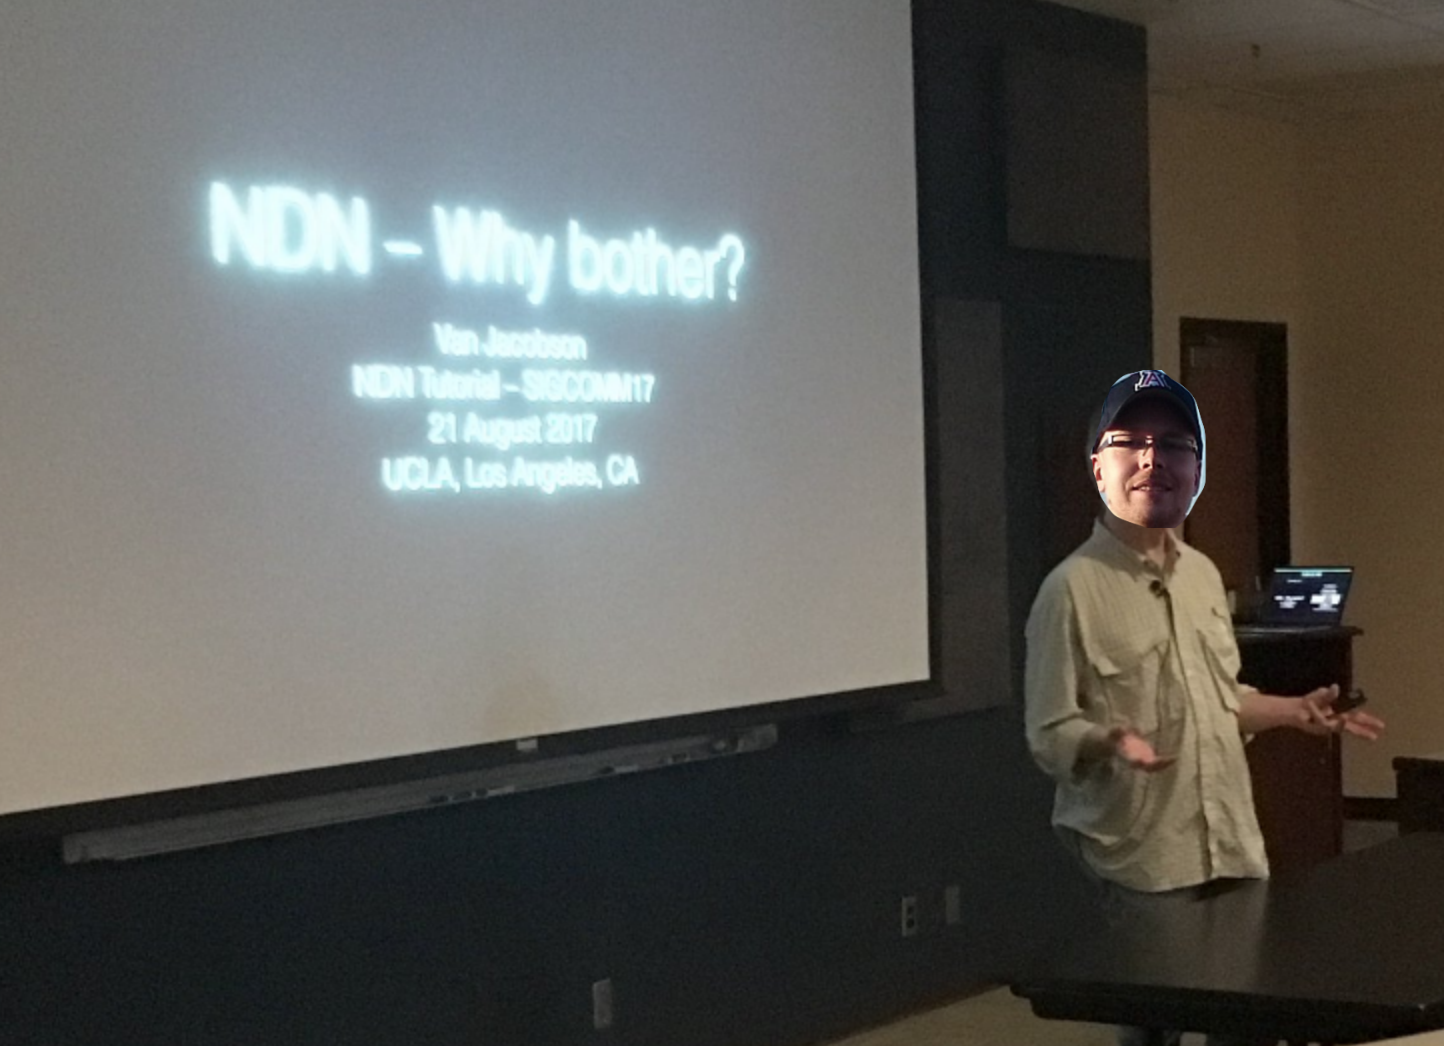
\includegraphics[width=\linewidth]{images/why_bother2.png}

\end{frame}


\begin{frame}{Why bother about \texttt{catchunks}/\texttt{putchunks}?}


\begin{enumerate}
\item Catchunks = First application new people use
\pause
\item Many larger applications built on ndnchunks
\pause
\item Improvements trickle down into SegmentFetcher
\end{enumerate}

\end{frame}


\begin{frame}{Some Reported Performance Issues}

\begin{enumerate}
\item Performance. on lossy, high-delay WiFi links

%\pause
%\item Poor performance with very low bw*delay product

\pause
\item Window decrease $>$ retransmissions? 

\pause
\item Catchunks exceeds maximum retries

\pause
\item Too many/too little cong. marks? (Unix, UDP)
\end{enumerate}

\end{frame}



\begin{frame}{Experiment Setup}

\textbf{Host --- Router (VM) --- Server (VM)}

\pause
\begin{itemize}
\item VMs: Virtualbox + mini-ndn
\item Traffic shaping (tc netem) at router!
\item Catchunks vs. Iperf3 (TCP)
\end{itemize}

\pause
%\vspace{1em}

\textbf{Variables:}
\begin{enumerate}
\item Bandwidth
\item Delay
\item Jitter
\item Buffer Queue Size (qdisc)
\item Link Loss
\end{enumerate}

\end{frame}


\begin{frame}[fragile]{Not the Problem: Delays $<$ 150ms}

BW=50Mbit, queueSize=300
\vspace{1em}

\begin{tabular}{rcc}
\toprule
\textbf{RTT} & \textbf{Catchunks (Mbps)} & \textbf{Iperf (Mbps)} \\ 
\midrule
2ms 	& 46.2  & 48.4 \\
50ms	& 45.3  & 47.4 \\
100ms & 30.2	& 32.4 \\
%200ms &  5.0  & 15.6 \\
\bottomrule
\end{tabular}

\end{frame}


\begin{frame}[fragile]{Not the Problem: Jitter}

BW=50Mbit, queueSize=300
\vspace{1em}

\begin{tabular}{rrcc}
\toprule
\textbf{RTT} & \textbf{Jitter} &  \textbf{Catchunks (Mbps)} & \textbf{Iperf (Mbps)} \\ 
\midrule
10ms 	& 1ms		& 45.2  & 48.1 \\
20ms 	& 2ms		& 43.3  & 45.4 \\
100ms	& 20ms	& 24.7  & 37.3 \\
%200ms &  5.0  & 15.6 \\
\bottomrule
\end{tabular}

\vspace*{1em}

$\Rightarrow$ Some difference, but not very large! (x1.5)

\end{frame}




\begin{frame}[fragile]{Not the Problem: Packet Loss}

BW=50Mbit, queueSize=300, delay=20ms
\vspace{1em}
 

\begin{tabular}{rcc}
\toprule
\textbf{Loss} & \textbf{Catchunks (Mbps)} & \textbf{Iperf (Mbps)} \\ 
\midrule
 .1\% & 38.4  & 38.3 \\
1.0\%		& 11.8  & 10.1 \\
5.0\%		&  3.5	&  3.5 \\
%200ms &  5.0  & 15.6 \\
\bottomrule
\end{tabular}

\vspace{1em}

%Loss = after L2 retransmissions. 5\% is very high!

\end{frame}


\begin{frame}[fragile]{Not the Problem: Delay + Jitter + Loss}

BW=50Mbps, qSize=300, delay=60ms, jitter=20ms, loss=1\%

\pause
\vspace{.5em}
 
\begin{tabbing}
\textbf{Catchunks:} \= 3.94 Mbps \\
\textbf{Iperf3:} \>    7.50 Mbps
\end{tabbing}
 
$\Rightarrow$ Higher difference, but still not very large! (x1.9)

\end{frame}



\begin{frame}[fragile]{The Problem: NFD Performance (1)}

\textbf{No Traffic Shaping}
\vspace*{-.5em}

\small
\begin{verbatim}
Time elapsed: 9620.52 milliseconds
Total size: 104858kB, 23832 segments
Goodput: 87.194912 Mbit/s
Total # of lost/retx segments: 829 (caused 40 window decr)
Packet loss rate: 3.36158%, cong marks: 10
RTT min/avg/max = 0.833/16.764/125.612 ms
\end{verbatim}

\pause
\begin{verbatim}
IPERF:
[ ID] Interval    Transfer    Bandwidth  Retr  Cwnd
[  4] 0.00-0.55s  100 MBytes  1.53 Gbps  92    348 KBytes       
\end{verbatim}

\pause
\textbf{CPU is the limiting factor:} \textbf{Router: 96\%,} Server: 80\% \\
$\Rightarrow$ \textbf{NFD,} buffer size, cong. marks, window adaptation?  

\end{frame}


\begin{frame}[fragile]{The Problem: Buffer Queue Size (2)}

BW=50Mbit, delay=20ms

\begin{tabular}{rcc}
\toprule
\textbf{Q (Pkts)} & \textbf{Catchunks (Mbps)} & \textbf{Iperf (Mbps)} \\ 
\midrule
  20  &  5.7  & 31.0 \\
  50	& 15.0  & 46.3 \\
 100	& 37.5  & 47.8 \\
 300	& 46.8	& 48.0 \\
1000	& 47.0	& 48.2 \\
%200ms &  5.0  & 15.6 \\
\bottomrule
\end{tabular}
\vspace*{1em}

Large difference: \textbf{5.4x lower throughput!}

\pause
Improves slightly with smaller chunk size (1.3KB)\\ 5.7 Mbps $\Rrightarrow$ 7.5 Mbps. 
\textbf{???}

\end{frame}



\begin{frame}[fragile]{The Problem: Delay $>$ 200ms (3)}

50MB file, BW=50Mbit, queueSize=1000
\vspace{1em}

\begin{tabular}{rcc}
\toprule
\textbf{RTT} & \textbf{Catchunks (Mbps)} & \textbf{Iperf (Mbps)} \\ 
\midrule
100ms &  11.8 & 44.1 \\
150ms &  12.4 & 44.6\\
200ms &  1.4  & 32.4 \\
300ms &  0.9  & 22.5 \\
400ms	&  2.2	&	16.6 \\
\bottomrule
\end{tabular}

\vspace*{1em}

Large difference: \textbf{25x lower throughput!}

\pause
\vspace*{.5em}

What's special about 200ms? $\Rightarrow$ \textbf{minRTO=200ms!} 

\end{frame}




\begin{frame}[fragile]{Hackathon Improvements: Better Statistics (1)}

\textbf{Measure spurious retransmissions!}
%\vspace*{-.5em}

\footnotesize
\begin{verbatim}
All segments have been received.
Time elapsed: 78861.7 milliseconds
Total # of segments received: 11916
Total size: 52428.8kB
Goodput: 5.318554 Mbit/s
\end{verbatim}
\begin{verbatim}
RTO Timeouts: 245 (caused 22 window decreases)
Retx segments: 49, skipped: 196
\end{verbatim}
\begin{verbatim}
Packet loss rate: 0.409528%
Total # of received congestion marks: 1
RTT min/avg/max = 201.598/207.656/261.004 ms
\end{verbatim}

\normalsize

\pause
Explains why sometimes \textbf{window decrease $>$ retx!}


%\begin{enumerate}
%\item Implement \textbf{TCP CUBIC} window adaptation
%\pause
%\item Look into \textbf{RTO calculation} (raise minRTO?)
%\pause
%\item Increase \# retries (Linux: 15)
%\pause
%\item Other options?
%\end{enumerate}

\end{frame}


\begin{frame}[fragile]{Hackathon Improvements: Increase RTO (2)}

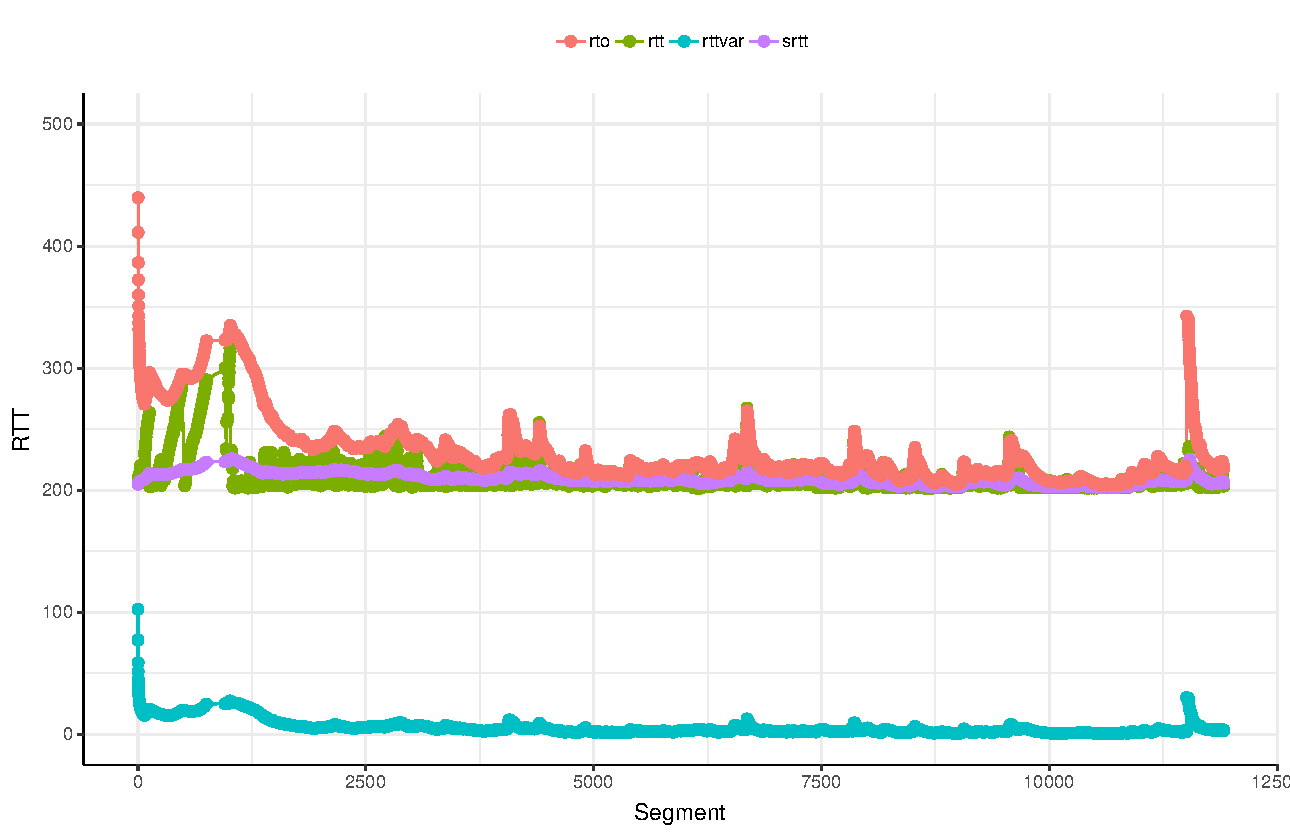
\includegraphics[width=\linewidth]{images/rtt_rto200ms.pdf}

$RTO = sRTT + k * varRTT$

\end{frame}


\begin{frame}[fragile]{Hackathon Improvements: Increase RTO (2)}

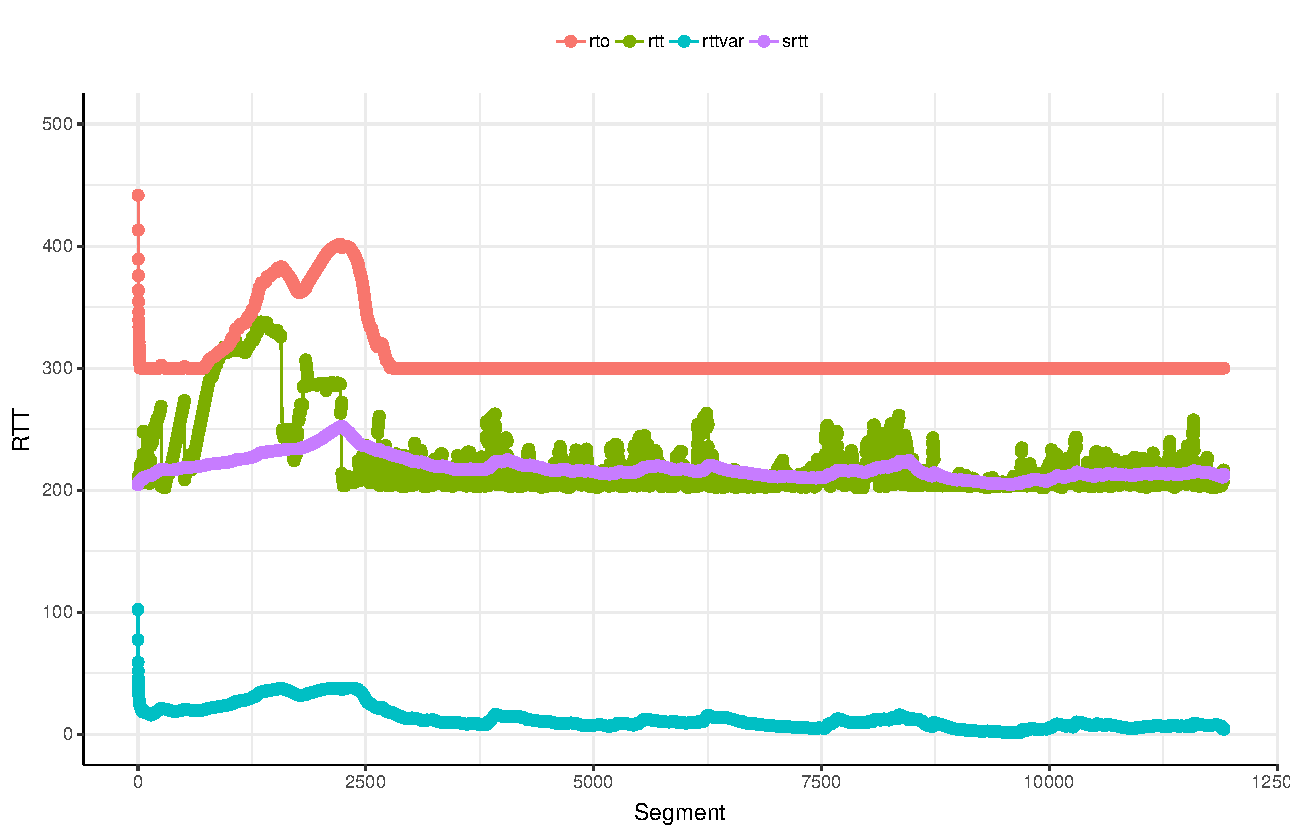
\includegraphics[width=\linewidth]{images/rtt_rto300ms.pdf}

Increase minRTO to 300ms

\end{frame}


\begin{frame}[fragile]{Hackathon Improvements: Increase RTO (2)}

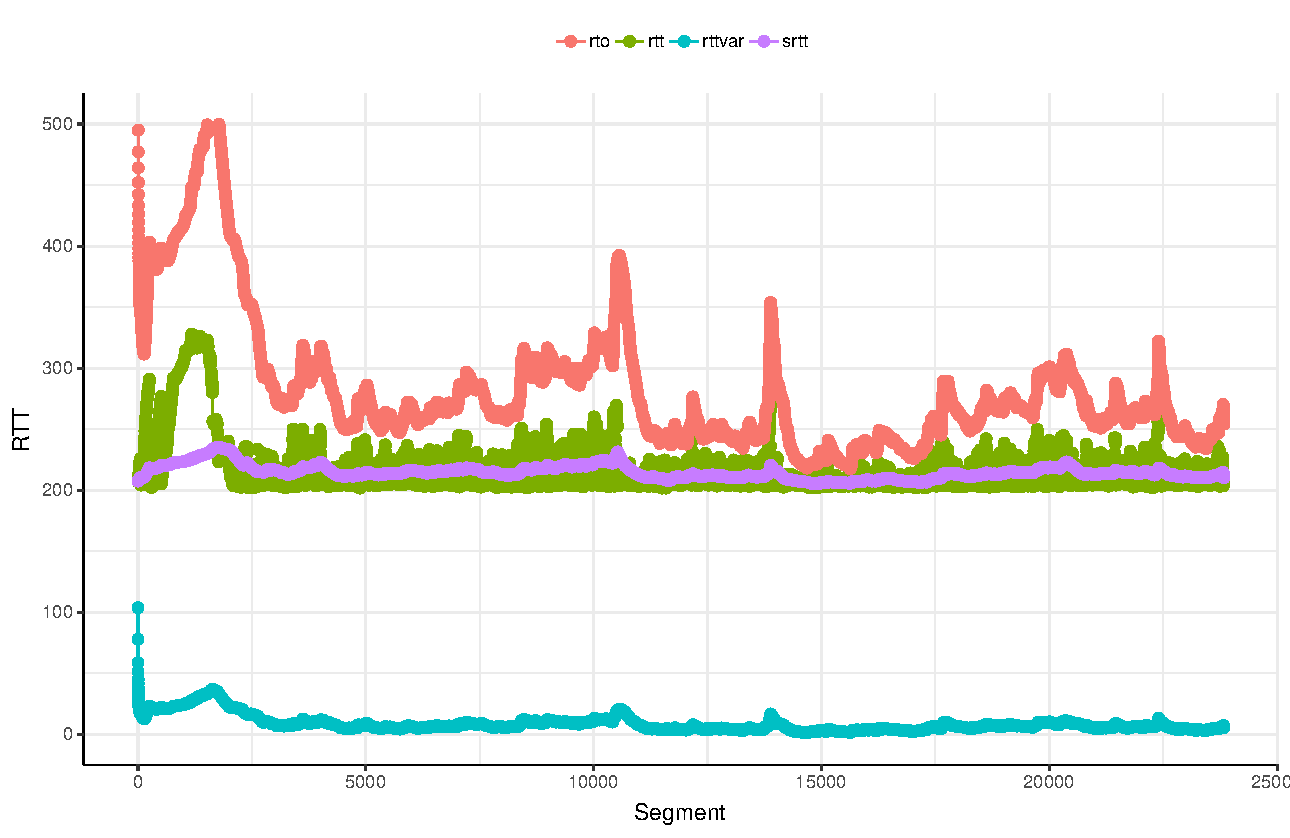
\includegraphics[width=\linewidth]{images/rtt_k8.pdf}

Increase \textbf{k=8.} 
TP:  5.6 Mbps $\Rightarrow$ \textbf{28.6 Mbps} (TCP: 34Mbps)

\end{frame}



\begin{frame}[fragile]{Hackathon Improvements: Impl. TCP CUBIC (3)}
Delay=400ms, 100MB file

\vspace*{1em}

\begin{tabular}{lccc}
\toprule
\textbf{Scen} & \textbf{TP (Mbps)} & \textbf{cwnd dec.} & \textbf{spur. rtx} \\ 
\midrule
AIMD, k=4 &   2.3 & 61 & 308  \\
CUBIC, k=4 &  8.8 & 27 & 260  \\
CUBIC, k=6 & 12.7 & 7 & 123  \\
CUBIC, k=8 & 14.6 & 7 & 5  \\
TCP 		  &  16.1 & - & -\\

\bottomrule
\end{tabular}

\end{frame}


\begin{frame}[fragile]{Small Improvements \& Open Problems}

\begin{enumerate}
\item Increase retry limit from 3 to \textbf{15!}

\pause
\item Look into \textbf{small buffer size} issue! 
\begin{itemize}
\item Timeouts: $>$ 1000 in NDN vs 80 in TCP
\item Increasing k \& CUBIC doesn't help
\end{itemize}

%\pause
%\item RTO Backoff mechanism doesn't work.
%\begin{itemize}
%\item 
%\end{itemize}


\pause
\item Tune congestion marks (UDP + Unix sockets)

\pause
\item Test with Mini-NDN WiFi
\end{enumerate}

\end{frame}


%% Last slide
\begin{frame}
	\frametitle{The End}
	\vspace{2cm}
	{\huge Any Questions?
%		Thank you for
%		your attention!\\
%		\vspace*{2em}
	}
	\vspace{2.5cm}  
	\begin{flushright}  
		Klaus Schneider, Saurab Dulal \\ 
%		\footnotesize{
%			\url{klaus@cs.arizona.edu} \\
%			\url{https://www.cs.arizona.edu/~klaus/} %\\ 
%		}
	\end{flushright}
\end{frame}




